Este fue un estudio monocéntrico doble-ciego controlado por placebo y de grupos paralelos y fue llevado a cabo en su totalidad en la Subdirección de Investigaciones Clínicas del Instituto Nacional de Psiquiatría Ramón de la Fuente Muñiz (INPRFM) en la Ciudad de México.\par
La investigación forma parte de un proyecto mayor financiado por CONACYT:
``Cambios en la estructura y conectividad funcional cerebrales relacionados a la mejoría clínica en pacientes con adicción a la cocaína después de un tratamiento con estimulación magnética transcraneal'',
clave S0008-2015-2-260971, bajo la dirección del doctor Eduardo Garza Villarreal y aprobado por el Comité de Ética del INPRFM (CEI/C/070/2016).

\section{Muestra}
Para el presente proyecto, tanto pacientes de la clínica de adicciones del INPRFM como externos que cumplieran con el diagnóstico de dependencia de cocaína (F14.2x) del DSM 5 \parencite{APA2013} fueron reclutados para participar en el ensayo clínico.\par
Se asignaron 46 sujetos aleatoriamente a los distintos grupos de estimulación (Figura \ref{fig:flow}).
Un grupo recibió estimulación sobre la corteza prefrontal dorsolateral izquierda y el otro, un protocolo sham de estimulación simulada sobre la misma área.

\subsection{Grupo control}
Para la realización del análisis transversal de pacientes adictos y controles sanos, los datos de neuroimagen de una submuestra de 45 sujetos sanos fueron retomados de la base de datos de un proyecto realizado con anterioridad en el INPRFM \parencite{Garza2017}.
Debido a que la cantidad total de los sujetos sanos de la base de datos de ese estudio es menor al número de participantes reclutados para nuestro proyecto, fue imposible parear ambos grupos.

\begin{figure}[H]
    \centering
    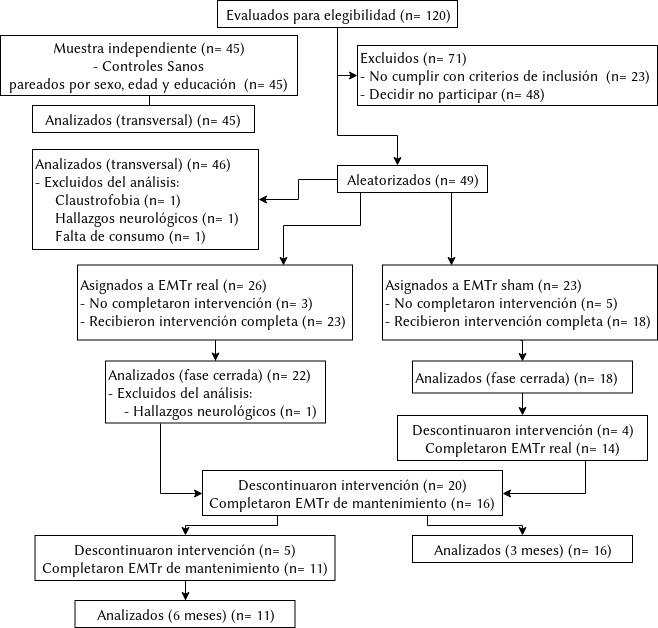
\includegraphics[width=\textwidth]{participantFlow}
    \caption{Diagrama de flujo de participantes}
    \label{fig:flow}
\end{figure}

\section{Criterios de selección}
Se siguieron los criterios de selección establecidos en el proyecto principal.
Estos fueron propuestos con la intención de disminuir la posibilidad de aparición de cualquier variable extraña y de seguir los lineamientos de seguridad tanto para la MRI como la EMTr.

\subsection{Criterios de inclusión}
Todos los participantes debían cumplir con los siguientes criterios para ser registrados en el estudio y ser asignados a uno de los grupos de investigación
\begin{enumerate*}[label=\emph{\alph*}), before=\unskip{: }, itemjoin={{; }}, itemjoin*={{, y }}]
    \item tener una edad mínima de 18 años y máxima de 50 años
    \item ser usuario de cocaína durante al menos dos  años, con un uso promedio actual mínimo de tres veces a la semana y periodos de abstinencia continua menores a un mes durante el último año
    \item poseer un nivel de lectura de al menos sexto año de primaria
    \item tener la capacidad de dar un consentimiento informado válido
    \item ser diestro
    \item tener un índice de masa corporal menor o igual a 30
    \item para las participantes del sexo femenino y en edad fértil, comprometerse a utilizar una forma médicamente aceptable\footnote{Píldora anticonceptiva, preparación hormonal, DIU o depósito (anillo, inyección, implante) y/o algún método anticonceptivo de barrera (diafragma, esponja, espermicida o condón).} de anticonceptivo y no quedar embarazada durante el estudio.
\end{enumerate*}

\subsection{Criterios de exclusión}
Los participantes fueron excluidos del estudio al presentar cualquiera de las siguientes características
\begin{enumerate*}[label=\emph{\alph*}), before=\unskip{: }, itemjoin={{; }}, itemjoin*={{, o }}]
    \item antecedentes personales o familiares de primer grado de cualquier trastorno neurológico, historia personal de neurocirugías previas o traumas craneoencefálicos que hayan producido pérdida de la conciencia
    \item tener alguno de los siguientes: marcapasos cardiaco, estimuladores neuronales, desfibriladores implantables, bomba de medicación implantada, líneas intracardiacas, implantes intracraneales (clips de aneurisma, derivaciones, estimuladores, implantes cocleares o electrodos) o cualquier objeto metálico dentro o cerca de la cabeza que no pueda ser retirado de forma segura
    \item esquirlas de metal o proyectiles metálicos en la cabeza o cuerpo
    \item uso actual de cualquier droga de investigación o de cualquier medicamento con acción proconvulsivante\footnote{Antidepresivos tricíclicos o neurolépticos que disminuyen el umbral convulsivo.}
    \item presión intracraneal aumentada
    \item historia de esquizofrenia, trastorno bipolar, manía o hipomanía
    \item historia de infarto de miocardio, angina de pecho, insuficiencia cardiaca congestiva, miocardiopatía, eventos vasculares cerebrales o ataque isquémico transitorio, o cualquier afección cardiaca actualmente bajo atención médica
    \item en mujeres, tener un potencial reproductivo y no utilizar una forma aceptable de anticoncepción, estar embarazadas o en lactancia
    \item cualquier historia de convulsiones
    \item dependencia actual (criterios DSM-5) a cualquier sustancia distinta a la cocaína o nicotina
    \item claustrofobia
    \item historia de infección por VIH o positivo a prueba de anticuerpos del VIH
\end{enumerate*}

\subsection{Criterios de eliminación}
Los criterios para suspender la participación de los sujetos durante el estudio fueron
\begin{enumerate*}[label=\emph{\alph*}), before=\unskip{: }, itemjoin={{; }}, itemjoin*={{, y }}]
    \item expresar deseo de dejar de participar
    \item presentar hallazgos radiológicos anormales que ameriten mayor atención fuera del estudio
    \item aparición de síntomas psicóticos relacionados con el trastorno adictivo
    \item presencia de una elevación anormal de ánimo relacionada a la aplicación de la EMTr.
\end{enumerate*}

\section{Fases del proyecto}
El presente proyecto de EMTr consiste en 4 etapas principales (Figura \ref{fig:txTMS}):
\begin{enumerate}[start=0,leftmargin=3\parindent,align=left,label=Etapa \arabic*:]
    \item Filtro de pacientes y etapa basal
    \item Dos semanas de tratamiento aleatorizado
    \item[Etapa 1-4:] Dos semanas de tratamiento real (únicamente integrantes de grupo sham)
    \item Tres meses de tratamiento de mantenimiento
    \item Seis meses de tratamiento de mantenimiento
\end{enumerate}

\begin{figure}[H]
    \centering
    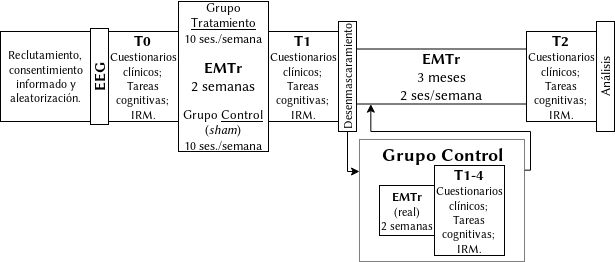
\includegraphics[width=\textwidth]{Des1}
    \caption{Linea de curso del tratamiento clínico de EMTr}
    \label{fig:txTMS}
\end{figure}

\subsubsection{Etapa 0}
Los participantes fueron reclutados dentro y fuera de la clínica de adicciones del INPRFM, buscando a todos aquellos que estuvieran interesados en un tratamiento para la dependencia a la cocaína.
Todos fueron entrevistados por un psiquiatra del instituto sobre los criterios de inclusión y exclusión.
En caso de ser admitidos al estudio, se les explicó completa y detalladamente las características principales del mismo y se les dio a firmar un consentimiento informado.
La asignación a grupos fue realizada por medio de un algoritmo aleatorizado por el director de la unidad y guardado en una memoria USB para cada sujeto que sería introducida directamente al resonador con tal de mantener el estado de doble-ciego.
La evaluación basal (T0) de los pacientes consistió en
\begin{enumerate*}[label=\emph{\alph*}), before=\unskip{: }, itemjoin={{; }}, itemjoin*={{, y }}]
    \item una entrevista clínica semi-estructurada aplicada por un psiquiatra
    \item una batería de escalas clínicas aplicada por un psiquiatra
    \item una batería de tareas cognitivas aplicadas por asistentes de investigación entrenados
    \item una prueba toxicológica de orina
    \item una corrida de MRI.
\end{enumerate*}
A todos los participantes se les aplicó un electroencefalograma para descartar cualquier actividad anómala que pudiera sugerir predisposición a un episodio convulsivo antes de iniciar con la fase de tratamiento.

\subsubsection{Etapa 1}
La primera fase de tratamiento consistió en 20 sesiones de EMTr real o sham a lo largo de 10 días hábiles consecutivos. Cada sesión fue aplicada por un técnico entrenado en la administración de EMTr. Tomó el umbral motor, ubicó la zona de estimulación y se encargo de aplicar los trenes de estimulación y estar al pendiente de posibles efectos adversos.
Los pacientes tuvieron un descanso de 30 minutos entre ambas sesiones.
Al finalizar, el técnico tomó un registro de cualquier molestia y se agendó la cita del siguiente día.\par
Una vez terminadas las 20 sesiones, los pacientes pasaron por otra evaluación (T1) clínica, de orina y MRI, antes de ser revelada su asignación de grupo.

\subsubsection{Etapa 1-4}
A todos aquellos participantes que llevaron estimulación sham se les ofreció continuar con un tratamiento de EMTr por otras 20 sesiones con las mismas características que el grupo de tratamiento real. Una vez concluidas las dos semanas de la fase abierta, una tercera evaluación clínica, de orina y MRI (T1-4) fue realizada.

\subsubsection{Etapa 2}
Esta etapa consistió en la primera fase de sesiones semanales de mantenimiento. Cuando los pacientes terminaron con las 20 sesiones de tratamiento real, se les citó semanalmente para dos sesiones de mantenimiento de EMTr por 10 semanas. Al completar los tres meses de la etapa basal, los pacientes tuvieron otra evaluación clínica, de orina y MRI (T2).

\subsubsection{Etapa 3}
Se continuó el mantenimiento bajo las mismas condiciones por otras 12 semanas hasta completar los seis meses transcurridos desde la etapa basal y llevar a cabo una última evaluación clínica, de orina y MRI (T3).

\section{Instrumentos}
\subsection{Medidas de \textit{craving} y recaída}
\begin{description}
    \item[CCQ-G] Cuestionario de \textit{Craving} de la Cocaína, versión general (\textit{Cocaine Craving Questionnaire, General}); escala que evalúa el deseo intenso hacia la droga de forma promedio en la última semana \parencite{Tiffany1993}.
    \item[CCQ-N] Cuestionario de \textit{Craving} a la Cocaína, versión actual (\textit{Cocaine Craving Questionnaire, Now}); escala que evalúa de forma presente el deseo intenso hacia la droga en el momento de aplicación \parencite{Tiffany1993}.
    \item[VAS] Escala Visual Análoga; escala visual análoga de \SI{100}{\milli\meter} utilizada para representar el \textit{craving} en el momento.
    \item[Línea de tiempo restrospectiva] Calendario de consumo como herramienta para medir el \emph{lapso} (por lo menos un evento de consumo con patrón diferente al basal) y \emph{relapso} (evento de consumo con el mismo patrón que el consumo basal).
\end{description}
\subsection{Medida de impulsividad}
\begin{description}
    \item[BIS-11] Escala de impulsividad de Barratt 11 (Barratt Impulsivity Scale 11); escala clínica que evalúa multidimensionalmente el índice de impulsividad \parencite{H.Patton1995,Salvo2013}.
\end{description}

\section{Estimulación magnética transcraneal repetitiva}
\subsection{Localización de la corteza prefrontal dorsolateral}
El objetivo de la estimulación cortical fue establecido tomando como base puntos de referencia craneales, utilizando la distancia teórica entre la región cortical objetivo y un punto en el cuero cabelludo determinado por EMT (procedimiento guiado funcionalmente) \parencite{Sparing2008}.
El área cortical motora izquierda fue el punto de referencia.
M1 fue determinada como la zona en donde hubiera una respuesta motora prominente en el dedo pulgar de la mano contralateral.
El umbral motor (MT) fue definido como la intensidad de estimulación menor que produjera una respuesta motora observable en al menos tres de cinco pulsos.
La localización de la corteza prefrontal dorsolateral fue \SI{5}{\centi\meter} anterior y \SI{2}{\centi\meter} lateral a M1 \parencite{Herwig2001a,Varnava2011a}.

\subsection{Estimulación real}
La EMTr fue aplicada con un estimulador rápido Magpro R-30 MagVenture (Medtronic, Dinamarca) equipado con una bobina MCF-P-B70 en forma de 8 y de \SI{75}{\milli\meter} de diámetro interno en cada espiral, con enfriamiento estático y capacidad de estimulación sham. \par
El centro de la bobina fue colocado sobre la corteza prefrontal dorsolateral izquierda con el asa a \SI{45}{\degree} relativos a la linea media-sagital. \par
La estimulación se aplicó en dos sesiones de EMTr a alta frecuencia (\SI{5}{\hertz}) en un mismo día separadas por un intervalo inter-sesión de \SI{30}{\minute}.
Cada sesión consistió en 50 trenes de \SI{10}{\second} con un intervalo inter-tren de \SI{1}{\minute} a 100\% del umbral motor, dando un total de 5000 pulsos divididos en dos sesiones de \SI{58}{\minute} y de 2500 pulsos.

\subsection{Estimulación sham}
La estimulación sham fue dada con el mismo estimulador y parámetros que la estimulación real. Sin embargo, la bobina fue colocada en su posición sham donde el sonido es idéntico a la estimulación real pero no dispara ningún pulso electromagnético.
A todos los sujetos durante las dos semanas de fase ciega se les colocó un electrodo en el músculo frontal sincronizado con el resonador con el fin de simular la sensación de la estimulación independientemente del grupo de tratamiento y mantener el doble-ciego.

\section{Imagen por resonancia magnética}
\subsection{Adquisición}
Tomamos las imágenes por resonancia magnética con un resonador Philips Ingenia de \SI{3}{\tesla} (Philips, EEUU) y una antena de cráneo de 32 canales. La corrida consistió en una secuencia estructural T1w de alta definición, una secuencia EPI de fMRI en estado de reposo, una secuencia de difusión HARDI-DWI y una secuencia experimental FAST-DKI. Para la presente investigación, solo utilizamos las secuencias funcional y la estructural.\par
Para la secuencia funcional, a los pacientes se les instruyó que se recostaran en el resonador moviéndose lo menos posible, que no pensaran en nada en específico y mantuvieran los ojos abiertos. Una cruz de fijación fue proyectada durante los \SI{10}{\minute} de secuencia funcional, pero se les explicó que no tenían que enfocarse en esta. \par
La fMRI fue tomada con una secuencia EPI (eco-planar) T2* con los siguientes parámetros
\begin{enumerate*}[label=\emph{\alph*}), before=\unskip{: }, itemjoin={{; }}, itemjoin*={{, y }}]
    \item TR = \SI{2}{\second}
    \item TE = \SI{30}{\milli\second}
    \item ángulo de inclinación de \SI{75}{\degree}
    \item 37 cortes de \SI{3.33}{\milli\meter} de grosor sin espacio entre corte
    \item FOV = \SI{240}{\milli\meter}
    \item matriz de \num{80x80}
    \item voxel de \SI[product-units=single]{3x3x3.33}{\milli\meter}.
\end{enumerate*}
Una secuencia \textit{fieldmap} fue tomada en dirección opuesta para el preprocesamiento.\par
La secuencia 3D de alta resolución T1w fue adquirida con los siguientes parámetros
\begin{enumerate*}[label=\emph{\alph*}), before=\unskip{: }, itemjoin={{; }}, itemjoin*={{, y }}]
    \item TR = \SI{7}{\milli\second}
    \item TE = \SI{3.5}{\milli\second}
    \item ángulo de inclinación de \SI{8}{\degree}
    \item 180 cortes de \SI{1}{\milli\meter} de grosor sin espacio entre corte
    \item FOV = \SI{240}{\milli\meter}
    \item matriz de \num{240x240}
    \item voxel de \SI[product-units=single]{1}{\milli\meter\cubed}.
\end{enumerate*}

\subsection{Manejo de datos}
Los datos de imagen fueron extraídos del formato \texttt{DICOM}, transformados a \texttt{NIfTI} y organizados en \texttt{BIDS} \parencite{Gorgolewski2016}.
La calidad de los datos fue evaluada con \texttt{MRIQC} \parencite{Esteban2017} para evaluar posibles artefactos de señal y/o movimiento. Los datos de neuroimagen de los controles sanos retomados de la investigación de \parencite{Garza2017} siguieron la misma línea de trabajo descrita a continuación.\par

\subsection{Preprocesamiento de datos}
Las imágenes fueron preprocesadas utilizando \texttt{FMRIPREP v1.4.1} \parencite{Esteban2019}, una herramienta basada en \texttt{Nipype} \parencite{Gorgolewski2011}.
Cada volumen de las imágenes T1w fue corregido por INU (no-uniformidad en intensidad) usando \texttt{N4BiasFieldCorrection v2.1.0} \parencite{Tustison2010} y se les removió el cráneo con \texttt{antsBrainExtraction.sh v2.1.0} (con la plantilla OASIS).
La normalización espacial a la plantilla ICBM 152 asimétrica no-lineal versión 2009c \parencite{Fonov2009} fue realizada por medio de un registro no-lineal con \texttt{antsRegistration} de \texttt{ANTs v2.1.0} \parencite{Avants2008}, usando versiones sin cráneo tanto del volumen T1w como de la plantilla.
La segmentación del tejido cerebral del líquido cefalorraquídeo (LCR), sustancia blanca (WM) y gris (GM) fue realizada en la imagen T1w sin cráneo usando \texttt{fast} de \texttt{FSL v.5.0.9} \parencite{Zhang2001}.\par
Los datos funcionales fueron corregidos por el tiempo de corte usando \texttt{3dTshift} de \texttt{AFNI v16.2.07} \parencite{Cox1996} y por movimiento con \texttt{mcflirt} (\texttt{FSL v5.0.9} \parencite{Jenkinson2002}.
Esto fue seguido por un corregistro al volumen T1w correspondiente usando un registro basado-en-límites \parencite{Greve2009} con seis grados de libertad, usando \texttt{bbregister} (\texttt{FreeSurfer v6.0.1}).
Las transformaciones para corregir movimiento, transformación BOLD-a-T1w y deformación T1w-a-plantilla (MNI) fueron concatenadas y aplicadas en un solo paso usando \texttt{antsApplyTransforms} \texttt{(ANTS v2.1.0)} usando interpolación Lanczos.\par
Una máscara para excluir señal con origen cortical fue obtenida erosionando la máscara del cerebro, asegurándose de que solo se contuvieran estructuras subcorticales.
Seis componentes tCompCor fueron entonces calculados incluyendo solo el top 5\% de voxeles variables dentro de la máscara subcortical.
Para aCompCor, seis componentes fueron calculados en el espacio T1w, después de su proyección al espacio nativo de cada corrida funcional.
El desplazamiento de marco (FD, \textit{frame-wise displacemente}) \parencite{Power2014} fue calculado para cada corrida funcional usando la implementación de \texttt{Nipype}.\par
Muchas operaciones internas de \texttt{FMRIPREP} usan \texttt{Nilearn} \parencite{Abraham2014}, principalmente dentro del flujo de trabajo del procesamiento BOLD. Para más detalles del trabajo de preprocesamiento ver \url{https://fmriprep.readthedocs.io/en/latest/workflows.html}.\par
Una vez obtenidas las matrices de regresiones de ruido de \texttt{FMRIPREP} los datos fueron preprocesados con la herramienta \texttt{xcpEngine} \parencite{Ciric2017}.
Debido a la naturaleza clínica de la muestra y las altas tasas de movimiento (medido por FD), utilizamos la estrategia de preprocesamiento de \textcite{Power2014} de 36 parámetros de regresión y \textit{scrubbing} (eliminación de los volúmenes que sobrepasen un umbral de FD establecido; en nuestro caso de \SI{0.5}{\milli\meter}).

\subsection{Construcción de redes}
Por medio de la misma herramienta de procesamiento \texttt{xcpEngine} se extrajeron las líneas de tiempo de la señal BOLD de cada uno de los 264 nodos del atlas funcional de \parencite{Power2011} basado en un meta-análisis de datos de fMRI de tareas.\par
Se utilizó \texttt{R v3.5.3} \parencite{R2019,Rstudio2018} para formar las matrices de adyacencia, obteniendo el coeficiente de correlación de Pearson $r$ de la señal BOLD entre cada una de las áreas de la parcelación.\par
Posteriormente con la intención de eliminar conexiones espúreas y disminuir el ruido dentro de las redes, aplicamos un método de umbralización de consenso donde se reconstruyen las matrices de adyacencia incluyendo solo las conexiones cuyo peso de conexión, o \emph{fuerza}, igualara o excediera un umbral grupal establecido:
\begin{equation}
    \label{eqn:threshold}
    w_{ij}=
    \begin{cases}
        w_{ij}, & \text{si}\ w_{ij} \geq \tau \enspace \text{en}\ (\frac{T}{100})m \\
        0, & \text{de otra forma}
    \end{cases}
\end{equation}
dado un umbral grupal $T$ (expresado como porcentaje) y una muestra de redes cerebrales $m$, una arista fue considerada en la reconstrucción de la matriz si sobrepasaba un umbral de conectividad $\tau$ en al menos $\frac{T}{100}m$ \parencite{DeReus2013}. \par
Para esta investigación los parámetros utilizados fueron $\tau = 0.25$ y $T = 50\%$; es decir, toda arista debía tener un valor de correlación igual o mayor a $0.25r$ en al menos la mitad de los integrantes del grupo para permanecer en la matriz reconstruida.\par
Del mismo modo, todas las auto-conexiones y conexiones negativas (anti-correlaciones funcionales) fueron retiradas de las matrices antes del análisis \parencite{Rubinov2010}.

\subsection{Medidas topológicas}
Una vez determinadas las matrices de adyacencia finales, los grafos de la red de conectividad funcional para cada sujeto fueron creados con la paquetería \texttt{brainGraph v2.2} \parencite{Watson2018}. Para cada grafo se extrajeron las siguientes medidas topológicas
\begin{enumerate*}[label=\emph{\alph*}), before=\unskip{: }, itemjoin={{; }}, itemjoin*={{, y }}]
    \item grado
    \item densidad
    \item coeficiente de agrupamiento
    \item longitud de camino característica
    \item eficiencia local
    \item eficiencia global
    \item escalar de mundo pequeño
\end{enumerate*}.

\subsection{Redes aleatorias}
Una vez construidos los grafos a partir de las matrices de adyacencia umbralizadas, con el fin de calcular las medidas de mundo pequeño, se crearon 300 redes con el mismo número de nodos y grado de conectividad siguiendo el procedimiento propuesto por \textcite{Maslov2002}. De estas redes se obtuvieron las medidas $L^w_g$ y $C^w_g$ para posteriormente calcular $\lambda_g$ (formula \ref{eqLambda}), $\gamma_g$ (formula \ref{eqGamma}) y el escalar de mundo pequeño $\sigma$ (formula \ref{eqSW}).

\section{Análisis de datos}
Todos los análisis estadísticos fueron hechos dentro del entorno de programación para \texttt{R} \texttt{RStudio} \parencite{Rstudio2018}.

Para el presente proyecto se realizaron cuatro análisis distintos.

\subsection{Análisis 1: Exploración transversal de controles}
Debido a la escasa investigación sobre la naturaleza de la topología de redes de conectividad funcional en sujetos con dependencia a la cocaína, se realizó una comparación transversal de las diferencias en las métricas de topología de red entre los 46 pacientes diagnosticados con dependencia a la cocaína que tuvieron una medición basal y los datos retomados de los 45 controles sanos.
En un análisis exploratorio observamos las distintas métricas de topología de red a lo largo de los distintos valores de $\tau$ de umbralizaje. Posteriormente se realizaron distintas regresiones lineales multivariadas para cada métrica de interés (fuerza, densidad, eficiencia local, eficiencia global y métrica de mundo pequeño). Las variables demográficas de edad, sexo y nivel educativo fueron incluidos como covariantes.

\subsection{Análisis 2: Fase cerrada}
Dado a la asignación grupal aleatoria del estudio, optamos por no explorar las diferencias demográficas y atribuirlas a efectos aleatorios.
Exploramos la relación entre los puntajes reportados en las distintas escalas clínicas por medio de una correlación de Pearson.
Ambos grupos (estimulación real y estimulación sham) fueron subdivididos a su vez por medio de la mediana del puntaje basal reportado por cada escala y por grupo con la intención de diferenciar los patrones de cambio de los pacientes que comenzaron el tratamiento con una sintomatología elevada de quienes mostraron una sintomatología leve.
La eficacia del tratamiento fue explorada utilizando regresiones lineales multivariadas para cada escala (VAS, CCQ-G, CCQ-N y BIS-11) usando el grupo de estimulación como predictor y las medidas clínicas basales como covariantes.
Los cambios en topología de red fueron analizados por medio de modelos de efectos mixtos. Para cada métrica de red, se realizó un modelo distinto buscando la interacción de fase de tratamiento y grupo de estimulación. Además se introdujeron las medidas clínicas y las variables demográficas de edad, sexo y nivel educativo como covariantes.

\subsection{Análisis 3: Fase abierta (tres meses)}
De forma exploratoria se analizaron los cambios observados posteriores a tres meses de sesiones semanales de mantenimiento en aquellos sujetos que llegaron hasta la fase T2.
Tanto las escalas clínicas como las métricas de red fueron exploradas por medio de modelos de efectos mixtos buscando la diferencia entre las distintas fases de la medición basal e incluyendo las variables demográficas de edad, sexo y nivel educativo como covariantes; para los modelos de las métricas topológicas además se incluyeron los puntajes clínicos.

\subsection{Análisis 4: Fase abierta (seis meses)}
Para obtener una medición más objetiva, se decidió separar el análisis longitudinal de mantenimiento en las mediciones a tres y seis meses. Para este segundo análisis, nos enfocamos únicamente en aquellos participantes que completaron todas las fases del estudio y exploramos sus cambios a lo largo de estas.
De igual forma que el análisis a tres meses, por medio de modelos de efectos mixtos se exploraron las diferencias con respecto a la medición basal incluyendo edad, sexo y nivel educativo como covariantes.

